\chapter{مروری بر کارهای گذشته، روش‌ها و ابزارهای موجود}
\section{مدل‌های کیفیتی}
با یک نگاه اجمالی بر منابعی همچون
\cite{wagner_software_2013}،
\cite{seffah_usability_2006}، 
\cite{pressman_software_2015}،
\cite{p._miguel_review_2014}
و همچنین
\cite{sommerville_software_2016}
که به بررسی و مقایسه تطبیقی مدل‌های کیفی پرداخته‌اند، به این نکته پی می‌بریم که صحبت از کیفیت و پژوهش در مورد مدل‌های کیفی از همان ابتدا و به صورت همزمان با پژوهش‌های مربوط به توسعه نرم‌افزار و متدولوژی‌ها مورد توجه بوده است.
در شکل
\ref{fig:qmodels}
ملاحظه می‌شود که از سال ۲۰۰۱، کم‌کم مدل‌های عام‌منظوره‌ای همچون مدل‌های مک‌کال و درومی
\LTRfootnote{Dromey}
کم‌رنگ‌تر شدند و شاهد معرفی شدن مدل‌های خاص‌منظوره بودیم.
\begin{figure}[H]
	\centering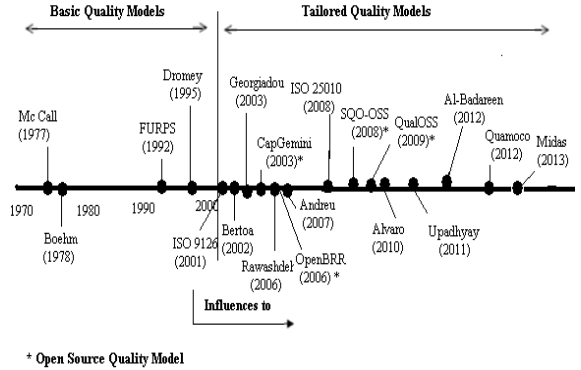
\includegraphics[width=10cm]{Resources/qmodels.PNG}
	\caption{خط زمانی ارائه برخی از مدل‌های کیفی
		\cite{p._miguel_review_2014}
	}
	\label{fig:qmodels}
\end{figure}
مدل‌های عام‌منظوره که در شکل با نام Basic شناخته می‌شوند، ابعاد کلی کیفیت نرم‌افزار را هدف قرار داده‌اند و تقریبا می‌توانند در هر نرم‌افزاری مورد استفاده قرار بگیرند؛ مدل‌های بعدی که ارائه شدند، روی ابعاد خاصی از سازمان یا محصول نرم‌افزاری تمرکز داشته‌اند. این مدل‌ها در نتیجه افزایش پیچیدگی محصولات نرم‌افزاری و فرایندهای سازمانی، برای استفاده در کاربردهای خاص و برای سازمان‌های خاص توسعه داده شدند
\cite{p._miguel_review_2014}.\\
در بررسی مدل‌های کیفی، مرجع
\cite{wagner_software_2013}
دسته‌بندی‌ای را ارائه داده است که بر اساس آن، مدل‌های کیفی را می‌توان به سه دسته سلسله‌مراتبی، مبتنی بر متامدل و همچنین مدل‌های ضمنی تقسیم‌بندی کرد که توضیحات هرکدام در ادامه به صورت مختصر قید شده است.
\subsection{مدل‌های سلسله‌مراتبی}
روش‌های Boehm
\cite{boehm_quantitative_1976}
و مک‌کال
\cite{mccall_factors_1977}
در ارائه مدل کیفی، تشابه زیادی باهم دارند؛ هر دو در خرد کردن مفهوم کیفیت، از یک روش سلسله‌مراتبی استفاده کردند و مطابق شکل
\ref{fig:heir}
کیفیت را به خصیصه‌های مشخصی (که از آن‌ها با نام فاکتورهای کیفیت یاد می‌شود) تقسیم کرده‌اند. این‌گونه مدل‌ها در طول زمان دچار تغییراتی شدند و تفاوت نحوه تقسیم‌بندی آن‌ها، تفاوت مدل‌ها را پدید آورده است.
\begin{figure}[H]
	\centering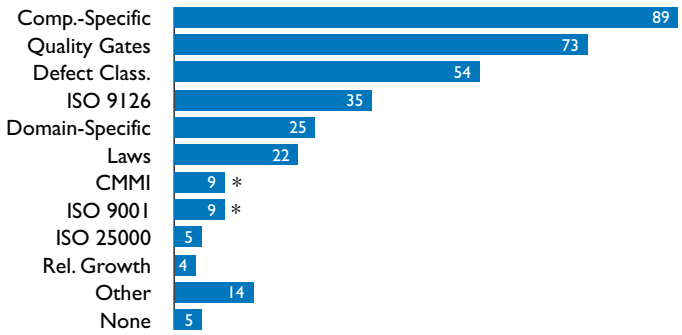
\includegraphics[width=9cm]{Resources/wagner.PNG}
	\caption{بررسی انواع مدل/رویه‌های کیفیتی استفاده شده در سازمان‌ها
		\cite{wagner_software_2012}
	}
	\label{fig:wagner}
\end{figure}
به تعبیر واگنر
\cite{wagner_software_2013}
رویکرد این نوع مدل‌های کیفی، خرد کردن کیفیت به معیارهای قابل اندازه‌گیری و در نهایت اندازه‌گیری و مقایسه آن‌هاست. همچنین واگنر در بررسی خود، از نقدهایی همچون «مبهم بودن برخی از این تقسیم‌بندی‌ها و شفاف نبودن آن‌ها به طور کامل» یاد می‌کند که از عوامل مهم ناکارآمدی برخی از آن‌هاست؛ همچنین وی در سال ۲۰۱۲ این نکته را متذکر شد که تنها کمتر از ۲۸٪ سازمان‌های فعال در حوزه نرم‌افزار، از مدل‌های استاندارد در تضمین کیفیت فعالیت‌ها و محصولاتشان استفاده می‌کنند و ۷۱٪ این سازمان‌ها، مدل‌های کیفی خود را از روی این مدل‌های کیفی، گلچین کرده و شخصی‌سازی می‌کنند
\cite{wagner_software_2012}.
\begin{figure}[H]
	\centering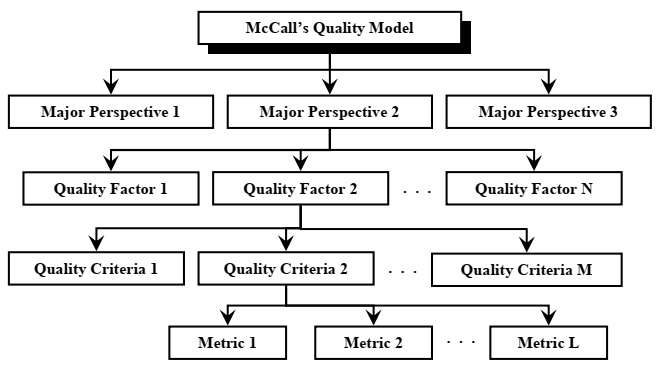
\includegraphics[width=11	cm]{Resources/heir.PNG}
	\caption{ساختار مدل کیفی مک‌کال به عنوان یک مدل کیفی سلسله‌مراتبی
		\cite{al-qutaish_quality_2010}
	}
	\label{fig:heir}
\end{figure}
همانطور که در شکل
\ref{fig:wagner}
مشاهده می‌شود، طی این بررسی، ۷۹ سازمان مدل‌های کیفیتی شخصی‌سازی‌شده توسط سازمان خود را در اولویت قرار داده و از آن‌ها استفاده می‌کنند. طبق اظهارات این بررسی و همچنین بسیاری از منابع دیگر همچون
\cite{pressman_software_2015} و
\cite{sommerville_software_2016}،
نیاز برای شخصی‌سازی مدل‌های کیفیتی استاندارد وجود دارد. چرا که این مدل‌های سلسله‌مراتبی، به صورت تجریدی بیان شده‌اند و نیازمند دقیق شدن روی متریک‌ها و روش‌های اندازه‌گیری هر متریک هستند.
\subsection{مدل‌های مبتنی بر متامدل}
با آشکار شدن این نیاز که می‌بایست مدل‌های پایه‌ای را بیشتر شفاف‌سازی کرد و آن‌ها را بر نیازمندی‌ها تطبیق بیشتری داد، ایده ارائه متامدل‌ها مطرح شد. متامدل در اصل مدلی از یک مدل کیفی است؛ قواعد و ساختارهایی که برای توصیف دقیق یک مدل کیفی نیاز داریم (همچون متریک‌ها و نحوه اندازه‌گیری آن‌ها)، توسط متامدل تعیین می‌گردند
\cite{deissenboeck_software_2009}.
به عبارت دیگر، توصیف اینکه چگونه یک مدل کیفی می‌تواند بر نیازمندی‌ها منطبق شود، به عهده متامدل است
\cite{wagner_software_2013}.
درومی به عنوان مثال، در سال ۱۹۹۵، متامدل نسبتا مفصلی ارائه داد که ذیل آن، میان مولفه‌های محصول نرم‌افزاری (که باید حامل کیفیت باشند - مانند کد منبع نرم‌افزار) و ویژگی‌های عملیاتی نرم‌افزار تفاوت و تمایز قائل شد
\cite{dromey_model_1995}.
\subsection{مدل‌های آماری و ضمنی}
این مدل‌ها سعی در ترجمه مفهوم اطمینان‌پذیری سخت‌افزار و استفاده آن در حوزه نرم‌افزار را دارند. ایده اصلی استفاده از این مدل‌ها، مشاهده خرابی‌ها در طول زمان و پیش‌بینی روند رخ دادن خرابی‌ها در آینده است. به منظور دستیابی به خصیصه‌های کیفیتی مشخصی که برای نیازهای توسعه محور بیان شده،در برخی از مدل‌ها سعی شده از داده‌های آماری برای به دست آوردن برخی از ویژگی‌ها و متریک‌ها استفاده شود.\\
به عنوان مثالی برای این نوع مدل‌ها می‌توان به مدل‌های
\textit{رشد اعتمادپذیری}\LTRfootnote{Reliability Growth Models}
\cite{musa_software_2004}
اشاره کرد. مدل‌هایی که از الگوریتم‌ها و روش‌های یادگیری ماشین برای تخمین موارد مختلف، از قبیل مولفه‌های آسیب‌پذیر و یا غیر کارا و مولفه‌هایی که دارای برخی از ویژگی‌های کیفی خاص نیستند نیز از این نوع‌اند که نمونه‌ای از این مدل‌ها در مرجع
\cite{neuhaus_predicting_2007}
تحت عنوان Vulture یاد شده؛ این مدل، از روش‌های یادگیری ماشین و از یک پایگاه دانش آسیب‌پذیری استفاده می‌کند تا در طول زمان و با گسترش نرم‌افزار، بتواند مولفه‌های آسیب‌پذیر نرم‌افزار را پیش‌بینی کند.\\
همچنین به تعبیر مرجع‌های
\cite{sommerville_software_2016}
و
\cite{wagner_software_2013}،
ابزارها و روش‌های مرور، داشبوردهای مدیریتی و مصورسازی داده، ابزارهای شناخت الگوی رخ‌داد خطا در کد منبع نرم‌افزار و چک‌لیست‌ها، که شاید در ظاهر به طور مستقیم ارتباطی با مدل‌های کیفی نداشته باشند، اما در نهایت به یک یا چند متریک کیفی در ذیل یک مدل کیفی ختم می‌شوند؛ این اشاره به مدل‌های کیفی به صورت ضمنی و غیرصریح بوده و اغلب به طور دقیق ارتباط خود با مدل‌ها را مشخص نکرده‌اند. در نتیجه‌ی ‌تمام موارد ذکر شده، تضمین و کنترل کیفیت به واسطه این سازوکارهای غیرصریح و مدل‌هایی که به طور ضمنی مطرح هستند، منجر به پیچیدگی بیشتر و سختی کار خواهد شد.

\section{تمرکز بر استفاده‌پذیری روی مدل‌های کیفیتی}
در جدول
\ref{tab:models}
مقایسه‌ای تطبیقی میان مدل‌های مطرح از سال ۱۹۷۰ تا ۲۰۱۱ انجام شده است که در انجام این مقایسه، به طور خاص، روی خصیصه استفاده‌پذیری این مدل‌ها تمرکز داشتیم. مدل‌های عام‌منظوره در کنار سایر مدل‌ها به مقایسه درآمده‌اند تا خصیصه‌های استفاده‌پذیری در هرکدام از آن‌ها بررسی شود؛ مدل‌های خاص‌منظوره به خاطر نیاز سازمان خاصی به وجود آمده‌اند که مشتریان مخصوص به خود را داشتند که در صورت تعویض محصول و مشتری و استفاده مدل مفروض در یک سازمان دیگر، الزاما به جواب بهینه منتهی نخواهد شد. در حقیقت ویژگی اصلی مدل‌های کیفیتی مبتنی بر متامدل و دلیل گستردگی آن‌ها، متفاوت بودن نیازهای مشتریان و شرایط سازمان‌هاست
\cite{sommerville_software_2016}.
\tiny
\begin{longtable}[c]{|c|c|c|c|c|}
	\caption{مقایسه تطبیقی مدل‌های کیفیتی ارائه شده با تمرکز بر استفاده‌پذیری}
	\label{tab:models} \\
	\hline
	ردیف & مدل کیفیتی ارائه شده  & سال ارائه & متریک‌های استفاده‌پذیری                                                                                                                              & مرجع \\ \hline
	\endfirsthead
	%
	\endhead
	%
1 & McCall & 1970 & Operability, Training, Communicativeness & \cite{mccall_factors_1977} \\ \hline
2 & Boehm & 1976 & Portability, Maintainability & \cite{boehm_quantitative_1976} \\ \hline
3 & \lr{IEEE 1061} & 1990 & Comprehensibility, Ease of Learning, Communicativeness & \cite{radatz_ieee_1990} \\ \hline
4 & Shackel & 1991 & Effectiveness, Learnability, Flexibility, Subjectively Pleasing & \cite{shackel_usability-context_1991} \\ \hline
5 & Bevan & 1991 & Type of Product, Type of User, Ease of Use, Acceptability & \cite{bevan_what_1991} \\ \hline
6 & FURPS & 1992 & Human Factors, Aesthetic, Documentation of the user, Material of Training & \cite{grady_practical_1992} \\ \hline
7 & Nielsen & 1994 & Learnability, Efficiency, Memorability, Errors, Satisfaction & \cite{nielsen_usability_1994} \\ \hline
8 & \lr{ISO 9126} & 2001 & Understandability, Learnability, Operability, Attractiveness, Usability Compliance & \cite{iso/iec_iso/iec_1991}  \\ \hline
10 & Bertoa & 2002 & Understandability, Learnability, Operability & \cite{bertoa_quality_2002} \\ \hline
11 & Georgiadou & 2003 & Support, Learnability, Documentation Update, Online Help, Consistency & \cite{georgiadou_gequamogeneric_2003} \\ \hline
13 & Abran & 2003 & Efficiency, Effectiveness, Satisfaction, Learnability, Security & \cite{abran_usability_2003} \\ \hline
14 & Bass & 2003 & Modifiability, Scalability, Reusability, Performance, Security & \cite{bass_linking_2003} \\ \hline
15 & Schneiderman & 2005 & \begin{tabular}[c]{@{}c@{}}Time to learn, Speed of Performance, Rate of Errors by users, Retention over time, Subjective\\ Satisfaction\end{tabular} & \cite{shneiderman_designing_2004}  \\ \hline
16 & Rawashdeh & 2006 & Understandability, Learnability, Operability, Complexity & \cite{rawashdeh_new_2006} \\ \hline
17 & \lr{ISO 25010} & 2008 & Approprateness, Recognizability, Learnability, Operability, User Error Protection, User Interface Aesthetics, Accessibility & \cite{noauthor_iso_nodate}  \\ \hline
18 & Alvaro & 2010 & Understandability, Learnability, Operability & \cite{alvaro_quality_2005, alvaro_software_2010} \\ \hline
19 & Alonso-Rios و بقیه & 2010 & Knowability, Operability, Efficiency, Robustness, Safety, Subjective Satisfaction & \cite{alonso-rios_usability:_2009} \\ \hline
20 & Dubey و بقیه & 2011 & Effectiveness, Efficiency, Satisfaction, Learnability & \cite{kumardubey_usability_2012} \\ \hline
\end{longtable}
	\normalsize
	شایان ذکر است که در همه مدل‌های ذکر شده، الزاما به استفاده‌پذیری به عنوان یک خصیصه اصلی در محصول اشاره نشده است؛ در بعضی از مدل‌ها همچون
	\lr{ISO 25010}
	استفاده‌پذیری یکی از سطوح اصلی بوده، در اولین سطح سلسه‌مراتبی مدل قرار داشته و جزئی از محصول نهایی است و در برخی دیگر همچون
	\lr{Boehm}،
	به طور صریح و مشخص به استفاده‌پذیری اشاره‌ای نشده است اما در فرآیندهای توسعه محصول روی آن توجه زیادی وجود دارد.\\
	همچنین از بررسی مدل‌های کیفیتی مختلف که صرفا برای توسعه سامانه‌های مبتنی بر وب این نتیجه برمی‌آید که هر متامدل می‌بایست در زمینه مربوط به خود مورد استفاده قرار گیرد و نه جای دیگر
	\cite{noauthor_measuringu:_2018}.
	نتیجه پیشین به این معنی است که در توسعه سامانه‌های مبتنی بر وب، محدوده کاربران، دانش قبلی آن‌ها، تخصص هرکدام، سن و سایر متغیرهای غیرقابل کنترل توسط توسعه‌دهنده نیز در استفاده‌پذیر بودن این سامانه تحت وب تاثیرگذار است؛ بنابراین در طراحی رابط کاربری هر سامانه مبتنی بر وب، می‌بایست به این نکات نیز توجه داشت و از آخرین توصیه‌های مربوط به توسعه این نوع سامانه‌ها استفاده کرد
	\cite{albert_measuring_2013}.
	از جمله این توصیه‌ها و پیشنهاد‌های طراحی، توصیه‌های گوگل برای ساخت اپلیکیشن‌های پیشرو\LTRfootnote{Progressive Web Applications}
	\cite{noauthor_progressive_nodate}
	است که جدیدا مطرح شده و طبق بررسی‌های انجام شده آینده‌ای روشن در انتظار این نوع از اپلیکیشن‌هاست.
	
\section{مطالعه استفاده‌پذیری و ارزیابی تجربه کاربری}
متریک‌هایی که در مطالعه استفاده‌پذیری و به طور خاص هنگام بررسی تجربه کاربری، اندازه‌گیری می‌شوند و مورد سنجش قرار می‌گیرند داده‌هایی را به دست ما می‌دهند که در بررسی و استفاده از این داده‌ها می‌توان دو رویکرد کلی داشت
\cite{albert_measuring_2013}:
ارزیابی خرد و ارزیابی کلان\RTLfootnote{
در سال ۱۹۸۶ و طی مقاله‌ای با عنوان «نقش ارزیابی مستمر و چرخشی در طراحی سیستم‌ها برای کیفیت»
\cite{hewett_role_1986}،
دو اصطلاح برای مطالعه تجربه کاربری و استفاده‌پذیری
\lr{Formative}
و
\lr{Summative}
مورد استفاده قرار گرفتند که هر دو از مفاهیم کلاس درسی برداشت شده‌اند؛ یک ارزیابی مستمر
(\lr{Formative})
به معنی پرسیدن سوال در سر کلاس درس توسط معلم بوده و به صورت تدریجی و خرد خرد است؛ در حالی که یک ارزیابی  کلان
(\lr{Summative})
مطالعه‌ای است که در انتهای هر بازه (مثلا هنگام امتحانات پایان‌ترم) و با برگزاری آزمونی خاص، ارزیابی‌ها انجام می‌شوند. در مقاله ذکر شده همچنین این مورد مطرح می‌شود که که ارزیابی مستمر و خرد برای رسیدن به دقت بالا در برآورد نیازهای مشتری، بهتر است.
}.\\
\begin{figure}
	\centering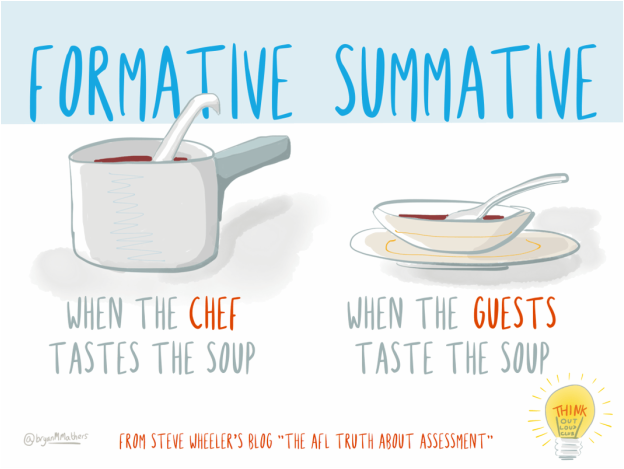
\includegraphics[width=10cm]{Resources/assessment.PNG}
	\caption{مثالی از دو نوع ارزیابی مختلف خرد و کلان
		\cite{noauthor_formative_nodate}
	}
	\label{fig:assessment}
\end{figure}
همانطور که در شکل
\ref{fig:assessment}
دیده می‌شود، می‌توان این دو نوع ارزیابی را به غذایی بدیل کرد که توسط آشپز و مشتری چشیده می‌شوند؛ آشپز در فرآیند پختن غذا به طور مرتب ممکن است غذا را بچشد تا در نهایت خروجی مطلوبی به دست مشتری برسد و غذا از کیفیت لازم برخوردار باشد. در حالی که مشتری در نهایت، محصول نهای را مشاهده می‌کند و صرفا نظر خود در مورد آن غذا و یا کیفیت رستوران را اعلام می‌کند. ذکر این نکته شایان ذکر است که به وضح می‌توان دریافت که هزینه اعمال تغییرات در صورت درخواست مشتری از آشپز زیاد خواهد بود؛ به طور مشابهی، در صورت عرضه محصول نرم‌افزاری، هزینه تعمیر یک خرابی به مراتب بیشتر از مرور در حین تولید است.
\subsection{ارزیابی خرد}
در یک مطالعه استفاده‌پذیری با رویکرد ارزیابی خرد، محقق به طور مستمر و به صورت دوره‌ای، محصول نهایی را مورد بررسی قرار می‌دهد و در تمامی مراحل تولید نواقص آن را سنجیده و کشف می‌کند و پیشنهاداتی برای رفع آن نواقص ارائه می‌دهد؛ این روند  تا آن جا ادامه پیدا می‌کند که نهایتا یک محصول تقریبا ایده‌آل و یا یک محصول خوب به اندازه کافی\LTRfootnote{
Good Enough
}
به دست آید. درواقع هدف در این نوع مطالعه هدف بهبود مستمر و رفع ایرادات محصول قبل از عرضه نهایی آن است؛ در نتیجه با بررسی فرآیندهای نرم‌افزاری و همچنین مطالعاتی از قبیل
\cite{sommerville_software_2016}،
\cite{krug_dont_2000} و
\cite{albert_measuring_2013}
به نظر می‌رسد که هرچه ارزیابی خرد زودتر رخ دهد، تاثیر بیشتری روی محصول نهایی و افزایش کیفیت آن خواهد داشت.\\
با اتخاذ این رویکرد، برخی از سوالاتی که می‌توان در فرایند طراحی پرسید عبارتند از:
\begin{itemize}
	\item 
	مهم‌ترین مواردی که کاربران را از رسیدن به اهدافشان منع می‌کند و یا به عدم کارایی آن‌ها می‌شود چیست؟
	\item 
	نقاط قوت و ضعف محصول از نقطه نظر کاربران چیست؟
	\item 
	اشتباهات متداول کاربران هنگام کار با محصول حول چه مواردی است؟
	\item 
	آیا بهبودهای مطرح شده توسط محققین تجربه کاربری، در هر نسخه از طراحی رابط کاربری، مورد استفاده و توجه قرار می‌گیرند؟
	\item 
	پس از عرضه نهایی محصول، چه مواردی در رابطه با استفاده‌پذیری به نظر می‌رسد که هنوز جای کار خواهد داشت؟
	
\end{itemize}
شایان ذکر است که در صورتی که فرصت اصلاح طراحی واسط کاربری وجود نداشته باشد، استفاده از این روش ارزیابی به نظر می‌رسد که کارایی چندانی نداشته باشد و بیشتر باعث هدررفت منابع شود.
\subsection{ارزیابی کلان}
در این روش، محقق همچون یک منتقد، محصول نهایی را از زوایای مختلف مورد بررسی قرار می‌دهد و حتی با محصول‌های دیگر مقایسه می‌کند تا نقدی بر آن وارد سازد. نکته حائز اهمیت این است که در اینجا محصول ارائه شده است و دیگر در فاز توسعه و تولید نیست. هدف از انجام این نوع ارزیابی، پی بردن به این نکته است که این محصول خاص چه‌قدر خوب می‌تواند به نیازمندی‌های کاربران پاسخ دهد و به چه میزان با آن‌ها هم‌جهت است. بر خلاف ارزیابی خرد، این روش، مبتنی بر اصول و قواعد و چک‌لیست‌های مشخصی است که در نهایت محصول با آن‌ها بررسی می‌شود. در مقایسه محصولات مختلف نیز مجددا این اصول و قواعد مبنا قرار می‌گیرند. با بررسی منابع مختلفی از قبیل
\cite{sommerville_software_2016} و
\cite{pressman_software_2015}
می‌توان به این نکته پی برد که سوالاتی از قبیل سوالات زیر بیشتر مناسب انجام این نوع ارزیابی هستند:
\begin{itemize}
	\item 
	آیا اهداف استفاده‌پذیری پروژه (مطرح شده در نیازمندی‌های پروژه) رعایت شده‌اند؟
	\item 
	استفاده‌پذیری کلی سیستم در چه سطحی است؟
	\item 
	نقاط ضعف و قوت محصول مورد نظر در مقایسه با سایر رقبا چیست و چگونه می‌توان در صورت داشتن ضعف، آن را ارتقا داد؟
	\item 
	آیا بهبودهای مطرح برای هر نسخه از نرم‌افزار، پس از عرضه نسخه جدید، اعمال می‌شوند؟
\end{itemize}
در نهایت فراموش نکنیم که همواره تغییر نیازمند صرف هزینه و زمان است؛‌ بنابراین در صورت استفاده از این روش ارزیابی می‌بایست در نظر داشت که برخی فعالیت‌های پسا ارزیابی نیز باید در پس ذهن مدیر پروژه باشد؛ چرا که ممکن است حتی در صورت نیاز پروژه‌ای برای برطرف کردن مشکلات استفاده‌پذیری یک سیستم تعریف شود که خود این پروژه هزینه‌بر باشد.
\subsection{اهداف کاربری}
سوالاتی همچون «آیا محصول مورد نظر نیاز روزانه کاربران را برآورده خواهد کرد و کاربران به طور متداول با این محصول نرم‌افزاری در ارتباط خواهند بود؟» و نیز «آیا کارایی کاربران و بهره‌وری آن‌ها در طول انجام یک وظیفه مشخص در هنگام کار با این نرم‌افزار مهم است؟ چگونه می‌توان آن را بهبود داد؟» به قسمتی از محصول توجه دارند که با نیازمندی‌های کاربر درگیر است. با بررسی‌ مراجعی همچون
\cite{albert_measuring_2013}،
\cite{noauthor_measuringu:_2018}،
\cite{hewett_role_1986} و
\cite{abran_usability_2003}
می‌توان به این نکته پی‌برد که همه این قبیل سوالات که به نیازهای ضمنی و نه الزاما صریح کاربر، در تعامل با رابط کاربری می‌پردازند، به دو متریک اساسی و قابل اندازه‌گیری از نیاز کاربران اشاره می‌کنند\RTLfootnote{
	ذکر این نکته خالی از لطف نیست که کارایی کاربر و رضایت کاربر در اینجا اشاره به دید کاربر به سامانه هدف دارند و نه اینکه متریک‌های اصلی مدل کیفیتی باشند. در اینجا کارایی و رضایت از دید کاربر و به عنوان نظر وی در مورد سامانه مورد نظر است.
}: کارایی\LTRfootnote{Performance} و رضایت کاربر\LTRfootnote{Satisfaction}.
\paragraph{کارایی}
به عنوان یک متریک کیفیتی به طور خاص در رابطه با تجربه کاربری، به اندازه‌گیری توانایی کاربران در انجام وظایف مشخصی می‌پردازد؛ در این راستا، اندازه‌گیری‌های جنبی نیز اهمیت زیادی پیدا می‌کنند. از جمله این اندازه‌گیری‌ها می‌توان به موارد زیر اشاره کرد که به طور غیر مستقیم در کارایی تاثیرگذار هستند:
\begin{itemize}
	\item 
	زمان سپری شده برای انجام وظیفه
	\item 
	میزان تلاش برای انجام وظیفه (برای مثال تعداد کلیک‌ها و یا توان ذهنی مصرف شده)
	\item 
	زمانی که طول می‌کشد تا کاربر با وظیفه آشنا شود و بدون صرف تلاش خاصی آن را انجام دهد (یادگیری)
\end{itemize}
اندازه‌گیری‌های مربوط به متریک کارایی یک رابط کاربری، اهمیت زیادی دارند چرا که اگر کاربران نتوانند وظایف اصلی در رابطه با تعامل با سیستم را به درستی و با موفقیت به انجام برسانند، در عمل محصول نرم‌افزاری به شکست منتهی شده است و یا حداقل رابط کاربری خوبی ندارد و امکان تعامل موفق کاربر وجود نخواهد داشت.
\paragraph{رضایت}
درواقع نظر نهایی کاربر در مورد تعاملش با سیستم است؛ قضاوتی که کاربر در مورد سیستم و نحوه تعاملش با آن می‌کند می‌تواند با جملات مختلفی مانند «استفاده از آن سخت/آسان بود»، «گیج‌کننده/ساده بود» و ... بیان شود. البته که این تعبیرات غیردقیق هستند اما می‌توان با اعطای درجه‌های آزادی خاصی به کاربران، در حین تعامل با سیستم برخی از متریک‌ها را از آن‌ها به طور خوداعلامی\LTRfootnote{Self-reported Metrics} از کاربران گزارش عددی گرفت؛ چه بسا که به گفته مراجعی همچون
\cite{albert_measuring_2013}،
\cite{alonso-rios_usability:_2009} و
\cite{seffah_usability_2006}
این متریک‌ها در سامانه‌های کاربردی مبتنی بر وب - که هدف اصلی این پروژه هستند - بسیار مهم و تاثیرگذارند. اما باید به این نکته توجه کرد که در محدوده سامانه‌های مبتنی بر وب، رضایت کاربر الزاما همیشه همراه با کارایی حداکثری وی در تعامل با سامانه نیست؛ فاکتورهای بسیاری از قبیل زیبایی و وجود تکنولوژی‌های مختلف، بر این رضایت تاثیر مستقیم دارند و چه بسا که کاربری با رضایت حداکثری از یک سامانه استفاده کند ولی کارایی عملیات وی بسیار پایین باشد.
\begin{figure}[H]
	\centering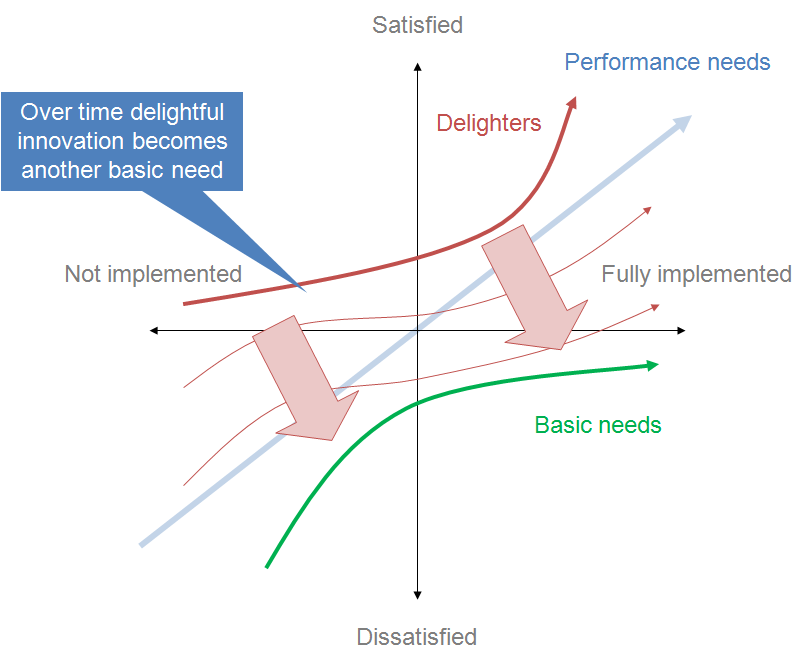
\includegraphics[width=13cm]{Resources/kano_model.PNG}
	\caption{مدل کانو که نشان‌دهنده ارتباط رضایت کاربر و ویژگی‌های محصول است
		\cite{noauthor_kano_2018}
	}
	\label{fig:kano}
\end{figure}
مدلی توسط آقای کانو در سال ۱۹۸۴
\cite{kano_attractive_1984}
برای تمییز دادن ویژگی‌های اشتیاق‌برانگیز و صریح و همچنین ویژگی‌های ضمنی و بایدی یک محصول، ارائه شد. طی این مدل، کیفیت محصول نهایی در گرو پنج دسته از نیازمندی‌های زیر است که رسیدن به هر دسته از این‌ها نیازمند اتخاذ سیاست‌های مختلف در طول ساخت محصول است:
\begin{itemize}
	\item 
	نیازمندی‌های بایدی: که مشتریان به طور ضمنی خواستار آن‌ها هستند و ممکن است صریحا بیان نشوند. به عنوان مثال اینکه یک سامانه کاربردی تحت وب همیشه با یک آدرس اینترنتی خاص
	\lr{URL}
	شناخته شود.
	\item
	نیازمندی‌های تک‌بعدی: که در صورت وجودشان کاربر احساس رضایتمندی و در صورت عدم وجودشان در محصول نهایی، کاربر احساس عدم رضایت از محصول را خواهد داشت. برای نمونه می‌توان به واکنش‌گرا بودن یک سامانه تحت وب روی پلتفرم موبایل اشاره کرد؛ که گفتنی است این روزها به یکی از ویژگی‌های اصلی موفقیت بسیاری از کسب‌وکارهای فعال در ایران تبدیل شده است.
	\item 
	نیازمندی‌های اشتیاق‌برانگیز: که در صورتی که به طور کامل پیاده‌سازی شوند، منجر به رضایتمندی کاربران خواهند شد ولی در صورت عدم پیاده‌سازی، رضایت کاربران از بین نخواهد رفت. به عنوان مثال اینکه یک سامانه پست الکترونیکی تحت وب\LTRfootnote{Webmail} در کنار لیست ایمیل‌های دریافتی، وضعیت آب‌وهوا و زمان فعلی و گزیده‌ای از اخبار را نشان دهد می‌تواند یک ویژگی اشتیاق برانگیز باشد.
	\item 
	نیازمندی‌های بی‌تفاوت: بودن و نبودنشان تفاوتی در رضایت مشتری نخواهد کرد. به عنوان مثال در بسیاری از پروژه‌های منتهی به یک سامانه کاربردی تحت وب، پلتفرم و زبان مورد استفاده برای توسعه سامانه، تفاوتی در رضایت مشتریان ایجاد نخواهد کرد.
	\item 
	نیازمندی‌های معکوس: به دسته‌ای از نیازمندی‌ها اشاره دارد که پرداختن بیش‌ازحد به آن‌ها باعث کاهش رضایت کاربران می‌شود. به عنوان مثال برخی از کاربران ممکن است از ابزارهایی که امکانات زیادی به آن‌ها در داشبورد مدیریتی می‌دهند خوششان بیاید و در مقابل برخی از کاربران از پیچیدگی بیش از حد ابزار گلایه کنند.
\end{itemize}
در شکل
\ref{fig:kano}
ملاحظه می‌شود که بسیاری از ویژگی‌های جذاب محصول که هنوز به عنوان نیازمندی مطرح هستند و هنوز پیاده‌سازی نشده‌اند و درنتجیه کاربر امکان انجام عملیات مورد نظر خود را ندارد، انگیزه‌ای برای ساخت سامانه هستند و پس از اینکه این ویژگی‌های عملیاتی (منحی قرمز رنگ) در محصول پدیدار می‌شوند، رضایت کاربران از محصول افزایش پیدا می‌کند؛ گرچه الزاما شاید این ویژگی‌ها، کارایی بالایی از دید کاربران نداشته باشند. به مرور زمان که فناوری پیشرفت می‌کند، نیازمندی‌های فعلی آهسته آهسته به باید‌های سامانه تبدیل می‌شوند (منحنی سبز رنگ).\\
همچنین در مرجع
\cite{sauerwein_kano_1996}
از خط آبی قابل مشاهده در شکل
\ref{fig:kano}،
به عنوان نیازمندی‌های تک‌بعدی یاد شده است که مشتری فقط به طور صریح و مشخص، این دسته از نیازمندی‌ها را مطرح می‌کند و بقیه نیازمندی‌ها معمولا به طور ضمنی مطرح می‌شوند.
نتیجه نهایی از دو بحث پیشین در مورد رضایت کاربر از سامانه و کارایی کاربر در تعامل با سامانه، اینکه این دو خصیصه الزاما دارای همبستگی خاصی نیستند؛ ولی همواره باید در اندازه‌گیری استفاده‌پذیری مدنظر قرار بگیرند چرا که طبق تعریف استفاده‌پذیری، در یک سیستم استفاده‌پذیر، کاربر می‌بایست در نهایت از سیستم راضی بوده باشد و تجربه کاربری خوبی داشته باشد.
\section{خصیصه‌های استفاده‌پذیری و اندازه‌گیری آن}
با بررسی مدل‌های کیفی 
\section{ابزارهای سنجش استفاده‌پذیری}
از جمله 





